\documentclass{extbook}[14pt]
\usepackage{multicol, enumerate, enumitem, hyperref, color, soul, setspace, parskip, fancyhdr, amssymb, amsthm, amsmath, bbm, latexsym, units, mathtools}
\everymath{\displaystyle}
\usepackage[headsep=0.5cm,headheight=0cm, left=1 in,right= 1 in,top= 1 in,bottom= 1 in]{geometry}
\usepackage{dashrule}  % Package to use the command below to create lines between items
\newcommand{\litem}[1]{\item #1

\rule{\textwidth}{0.4pt}}
\pagestyle{fancy}
\lhead{}
\chead{Answer Key for Progress Quiz 3 Version A}
\rhead{}
\lfoot{}
\cfoot{}
\rfoot{Fall 2020}
\begin{document}
\textbf{This key should allow you to understand why you choose the option you did (beyond just getting a question right or wrong). \href{https://xronos.clas.ufl.edu/mac1105spring2020/courseDescriptionAndMisc/Exams/LearningFromResults}{More instructions on how to use this key can be found here}.}

\textbf{If you have a suggestion to make the keys better, \href{https://forms.gle/CZkbZmPbC9XALEE88}{please fill out the short survey here}.}

\textit{Note: This key is auto-generated and may contain issues and/or errors. The keys are reviewed after each exam to ensure grading is done accurately. If there are issues (like duplicate options), they are noted in the offline gradebook. The keys are a work-in-progress to give students as many resources to improve as possible.}

\rule{\textwidth}{0.4pt}

\begin{enumerate}\litem{
Which of the following equations \textit{could} be of the graph presented below?

\begin{center}
    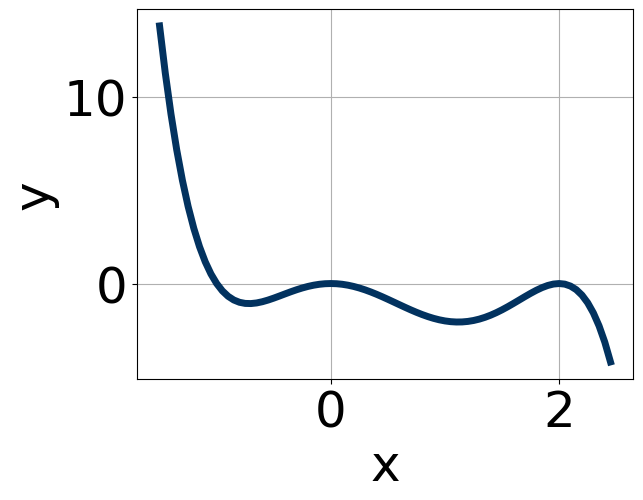
\includegraphics[width=0.5\textwidth]{../Figures/polyGraphToFunctionA.png}
\end{center}



The solution is \( 7(x + 4)^{4} (x - 1)^{6} (x - 3)^{6} \), which is option B.\begin{enumerate}[label=\Alph*.]
\item \( -5(x + 4)^{4} (x - 1)^{4} (x - 3)^{6} \)

This corresponds to the leading coefficient being the opposite value than it should be.
\item \( 7(x + 4)^{4} (x - 1)^{6} (x - 3)^{6} \)

* This is the correct option.
\item \( 2(x + 4)^{6} (x - 1)^{10} (x - 3)^{7} \)

The factor $(x - 3)$ should have an even power.
\item \( 6(x + 4)^{6} (x - 1)^{5} (x - 3)^{11} \)

The factors $(x - 1)$ and $(x - 3)$ should both have even powers.
\item \( -17(x + 4)^{10} (x - 1)^{10} (x - 3)^{11} \)

The factor $(x - 3)$ should have an even power and the leading coefficient should be the opposite sign.
\end{enumerate}

\textbf{General Comment:} General Comments: Draw the x-axis to determine which zeros are touching (and so have even multiplicity) or cross (and have odd multiplicity).
}
\litem{
Construct the lowest-degree polynomial given the zeros below. Then, choose the intervals that contain the coefficients of the polynomial in the form $x^3+bx^2+cx+d$.
\[ 5 + 4 i \text{ and } 2 \]
The solution is \( x^{3} -12 x^{2} +61 x -82 \), which is option C.\begin{enumerate}[label=\Alph*.]
\item \( b \in [1, 8], c \in [-7.98, -6.69], \text{ and } d \in [9.7, 10.6] \)

$x^{3} + x^{2} -7 x + 10$, which corresponds to multiplying out $(x -5)(x -2)$.
\item \( b \in [1, 8], c \in [-6.23, -5.01], \text{ and } d \in [6.5, 9.7] \)

$x^{3} + x^{2} -6 x + 8$, which corresponds to multiplying out $(x -4)(x -2)$.
\item \( b \in [-15, -10], c \in [60.98, 61.96], \text{ and } d \in [-84.3, -79.9] \)

* $x^{3} -12 x^{2} +61 x -82$, which is the correct option.
\item \( b \in [8, 15], c \in [60.98, 61.96], \text{ and } d \in [80.1, 83.9] \)

$x^{3} +12 x^{2} +61 x + 82$, which corresponds to multiplying out $(x-(5 + 4 i))(x-(5 - 4 i))(x + 2)$.
\item \( \text{None of the above.} \)

This corresponds to making an unanticipated error or not understanding how to use nonreal complex numbers to create the lowest-degree polynomial. If you chose this and are not sure what you did wrong, please contact the coordinator for help.
\end{enumerate}

\textbf{General Comment:} Remember that the conjugate of $a+bi$ is $a-bi$. Since these zeros always come in pairs, we need to multiply out $(x-(5 + 4 i))(x-(5 - 4 i))(x-(2))$.
}
\litem{
Construct the lowest-degree polynomial given the zeros below. Then, choose the intervals that contain the coefficients of the polynomial in the form $ax^3+bx^2+cx+d$.
\[ \frac{-2}{3}, \frac{4}{5}, \text{ and } \frac{-1}{4} \]
The solution is \( 60x^{3} +7 x^{2} -34 x -8 \), which is option D.\begin{enumerate}[label=\Alph*.]
\item \( a \in [58, 61], b \in [-8, -6], c \in [-40, -31], \text{ and } d \in [1, 11] \)

$60x^{3} -7 x^{2} -34 x + 8$, which corresponds to multiplying out $(3x -2)(5x + 4)(4x -1)$.
\item \( a \in [58, 61], b \in [14, 25], c \in [-31, -29], \text{ and } d \in [-10, -6] \)

$60x^{3} +23 x^{2} -30 x -8$, which corresponds to multiplying out $(3x + 3)(5x + 5)(4x -4)$.
\item \( a \in [58, 61], b \in [-73, -63], c \in [5, 13], \text{ and } d \in [1, 11] \)

$60x^{3} -73 x^{2} +10 x + 8$, which corresponds to multiplying out $(3x + 3)(5x -5)(4x -4)$.
\item \( a \in [58, 61], b \in [-4, 10], c \in [-40, -31], \text{ and } d \in [-10, -6] \)

* $60x^{3} +7 x^{2} -34 x -8$, which is the correct option.
\item \( a \in [58, 61], b \in [-4, 10], c \in [-40, -31], \text{ and } d \in [1, 11] \)

$60x^{3} +7 x^{2} -34 x + 8$, which corresponds to multiplying everything correctly except the constant term.
\end{enumerate}

\textbf{General Comment:} To construct the lowest-degree polynomial, you want to multiply out $(3x + 2)(5x -4)(4x + 1)$
}
\litem{
Which of the following equations \textit{could} be of the graph presented below?

\begin{center}
    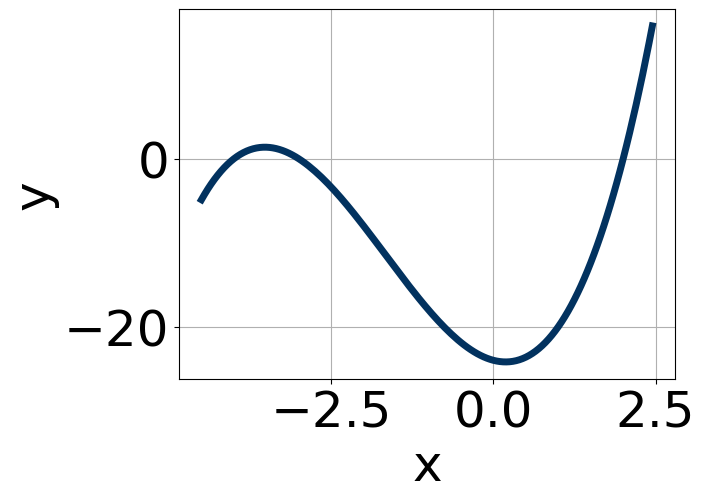
\includegraphics[width=0.5\textwidth]{../Figures/polyGraphToFunctionCopyA.png}
\end{center}



The solution is \( 16(x + 3)^{5} (x - 2)^{11} (x + 4)^{7} \), which is option A.\begin{enumerate}[label=\Alph*.]
\item \( 16(x + 3)^{5} (x - 2)^{11} (x + 4)^{7} \)

* This is the correct option.
\item \( 4(x + 3)^{8} (x - 2)^{10} (x + 4)^{11} \)

The factors $-3$ and $2$ have have been odd power.
\item \( -16(x + 3)^{11} (x - 2)^{5} (x + 4)^{5} \)

This corresponds to the leading coefficient being the opposite value than it should be.
\item \( -20(x + 3)^{6} (x - 2)^{5} (x + 4)^{11} \)

The factor $(x + 3)$ should have an odd power and the leading coefficient should be the opposite sign.
\item \( 20(x + 3)^{6} (x - 2)^{7} (x + 4)^{7} \)

The factor $-3$ should have been an odd power.
\end{enumerate}

\textbf{General Comment:} General Comments: Draw the x-axis to determine which zeros are touching (and so have even multiplicity) or cross (and have odd multiplicity).
}
\litem{
Construct the lowest-degree polynomial given the zeros below. Then, choose the intervals that contain the coefficients of the polynomial in the form $ax^3+bx^2+cx+d$.
\[ \frac{3}{2}, \frac{2}{5}, \text{ and } \frac{3}{4} \]
The solution is \( 40x^{3} -106 x^{2} +81 x -18 \), which is option C.\begin{enumerate}[label=\Alph*.]
\item \( a \in [38, 49], b \in [38, 47], c \in [-40, -29], \text{ and } d \in [-23, -17] \)

$40x^{3} +46 x^{2} -33 x -18$, which corresponds to multiplying out $(2x + 2)(5x + 5)(4x -4)$.
\item \( a \in [38, 49], b \in [13, 17], c \in [-58, -53], \text{ and } d \in [13, 20] \)

$40x^{3} +14 x^{2} -57 x + 18$, which corresponds to multiplying out $(2x + 2)(5x -5)(4x -4)$.
\item \( a \in [38, 49], b \in [-108, -98], c \in [72, 89], \text{ and } d \in [-23, -17] \)

* $40x^{3} -106 x^{2} +81 x -18$, which is the correct option.
\item \( a \in [38, 49], b \in [-108, -98], c \in [72, 89], \text{ and } d \in [13, 20] \)

$40x^{3} -106 x^{2} +81 x + 18$, which corresponds to multiplying everything correctly except the constant term.
\item \( a \in [38, 49], b \in [103, 112], c \in [72, 89], \text{ and } d \in [13, 20] \)

$40x^{3} +106 x^{2} +81 x + 18$, which corresponds to multiplying out $(2x + 3)(5x + 2)(4x + 3)$.
\end{enumerate}

\textbf{General Comment:} To construct the lowest-degree polynomial, you want to multiply out $(2x -3)(5x -2)(4x -3)$
}
\litem{
Describe the end behavior of the polynomial below.
\[ f(x) = 2(x + 6)^{5}(x - 6)^{8}(x - 4)^{3}(x + 4)^{3} \]
The solution is the graph below, which is option D.
\begin{center}
    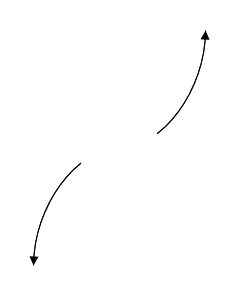
\includegraphics[width=0.3\textwidth]{../Figures/polyEndBehaviorDA.png}
\end{center}\begin{enumerate}[label=\Alph*.]
\begin{multicols}{2}
\item 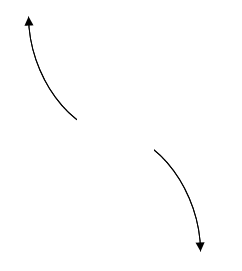
\includegraphics[width = 0.3\textwidth]{../Figures/polyEndBehaviorAA.png}
\item 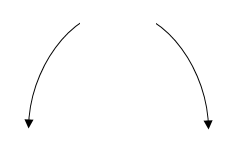
\includegraphics[width = 0.3\textwidth]{../Figures/polyEndBehaviorBA.png}
\item 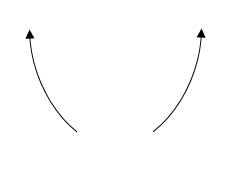
\includegraphics[width = 0.3\textwidth]{../Figures/polyEndBehaviorCA.png}
\item 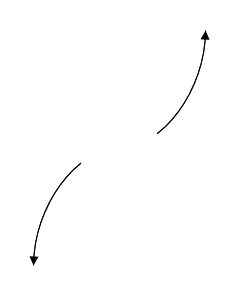
\includegraphics[width = 0.3\textwidth]{../Figures/polyEndBehaviorDA.png}
\end{multicols}\item None of the above.\end{enumerate}
\textbf{General Comment:} Remember that end behavior is determined by the leading coefficient AND whether the \textbf{sum} of the multiplicities is positive or negative.
}
\litem{
Describe the zero behavior of the zero $x = -7$ of the polynomial below.
\[ f(x) = 3(x - 7)^{4}(x + 7)^{7}(x - 4)^{4}(x + 4)^{7} \]
The solution is the graph below, which is option A.
\begin{center}
    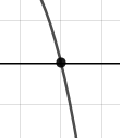
\includegraphics[width=0.3\textwidth]{../Figures/polyZeroBehaviorAA.png}
\end{center}\begin{enumerate}[label=\Alph*.]
\begin{multicols}{2}
\item 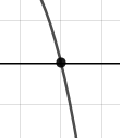
\includegraphics[width = 0.3\textwidth]{../Figures/polyZeroBehaviorAA.png}
\item 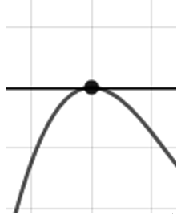
\includegraphics[width = 0.3\textwidth]{../Figures/polyZeroBehaviorBA.png}
\item 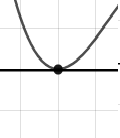
\includegraphics[width = 0.3\textwidth]{../Figures/polyZeroBehaviorCA.png}
\item 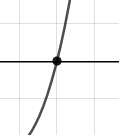
\includegraphics[width = 0.3\textwidth]{../Figures/polyZeroBehaviorDA.png}
\end{multicols}\item None of the above.\end{enumerate}
\textbf{General Comment:} You will need to sketch the entire graph, then zoom in on the zero the question asks about.
}
\litem{
Describe the zero behavior of the zero $x = 3$ of the polynomial below.
\[ f(x) = 5(x - 9)^{4}(x + 9)^{3}(x + 3)^{9}(x - 3)^{8} \]
The solution is the graph below, which is option C.
\begin{center}
    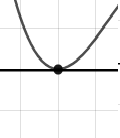
\includegraphics[width=0.3\textwidth]{../Figures/polyZeroBehaviorCopyCA.png}
\end{center}\begin{enumerate}[label=\Alph*.]
\begin{multicols}{2}
\item 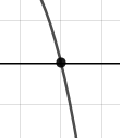
\includegraphics[width = 0.3\textwidth]{../Figures/polyZeroBehaviorCopyAA.png}
\item 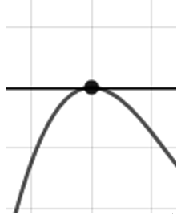
\includegraphics[width = 0.3\textwidth]{../Figures/polyZeroBehaviorCopyBA.png}
\item 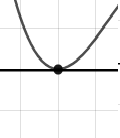
\includegraphics[width = 0.3\textwidth]{../Figures/polyZeroBehaviorCopyCA.png}
\item 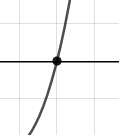
\includegraphics[width = 0.3\textwidth]{../Figures/polyZeroBehaviorCopyDA.png}
\end{multicols}\item None of the above.\end{enumerate}
\textbf{General Comment:} You will need to sketch the entire graph, then zoom in on the zero the question asks about.
}
\litem{
Describe the end behavior of the polynomial below.
\[ f(x) = -8(x + 9)^{2}(x - 9)^{3}(x - 4)^{2}(x + 4)^{2} \]
The solution is the graph below, which is option A.
\begin{center}
    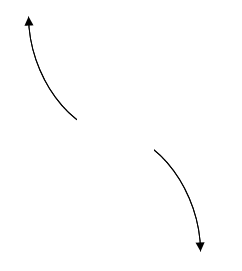
\includegraphics[width=0.3\textwidth]{../Figures/polyEndBehaviorCopyAA.png}
\end{center}\begin{enumerate}[label=\Alph*.]
\begin{multicols}{2}
\item 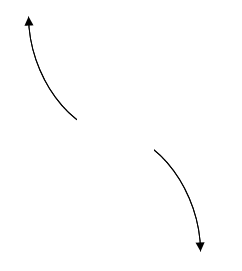
\includegraphics[width = 0.3\textwidth]{../Figures/polyEndBehaviorCopyAA.png}
\item 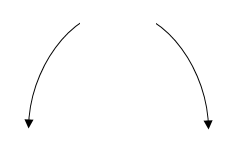
\includegraphics[width = 0.3\textwidth]{../Figures/polyEndBehaviorCopyBA.png}
\item 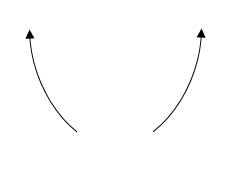
\includegraphics[width = 0.3\textwidth]{../Figures/polyEndBehaviorCopyCA.png}
\item 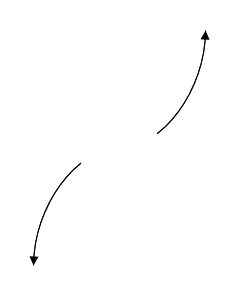
\includegraphics[width = 0.3\textwidth]{../Figures/polyEndBehaviorCopyDA.png}
\end{multicols}\item None of the above.\end{enumerate}
\textbf{General Comment:} Remember that end behavior is determined by the leading coefficient AND whether the \textbf{sum} of the multiplicities is positive or negative.
}
\litem{
Construct the lowest-degree polynomial given the zeros below. Then, choose the intervals that contain the coefficients of the polynomial in the form $x^3+bx^2+cx+d$.
\[ 3 - 3 i \text{ and } 1 \]
The solution is \( x^{3} -7 x^{2} +24 x -18 \), which is option A.\begin{enumerate}[label=\Alph*.]
\item \( b \in [-15, -5], c \in [18, 28], \text{ and } d \in [-19.7, -15.4] \)

* $x^{3} -7 x^{2} +24 x -18$, which is the correct option.
\item \( b \in [1, 2], c \in [-6, -1], \text{ and } d \in [1.5, 3.1] \)

$x^{3} + x^{2} -4 x + 3$, which corresponds to multiplying out $(x -3)(x -1)$.
\item \( b \in [3, 8], c \in [18, 28], \text{ and } d \in [17.8, 20.6] \)

$x^{3} +7 x^{2} +24 x + 18$, which corresponds to multiplying out $(x-(3 - 3 i))(x-(3 + 3 i))(x + 1)$.
\item \( b \in [1, 2], c \in [-2, 7], \text{ and } d \in [-3.5, 0.4] \)

$x^{3} + x^{2} +2 x -3$, which corresponds to multiplying out $(x + 3)(x -1)$.
\item \( \text{None of the above.} \)

This corresponds to making an unanticipated error or not understanding how to use nonreal complex numbers to create the lowest-degree polynomial. If you chose this and are not sure what you did wrong, please contact the coordinator for help.
\end{enumerate}

\textbf{General Comment:} Remember that the conjugate of $a+bi$ is $a-bi$. Since these zeros always come in pairs, we need to multiply out $(x-(3 - 3 i))(x-(3 + 3 i))(x-(1))$.
}
\end{enumerate}

\end{document}